\documentclass{article}
\usepackage{amsthm}
\usepackage{amsmath}
\usepackage{graphicx}
\usepackage{tikz}
\usepackage{wasysym}

\newtheorem{problem}{Problem}

\begin{document}
\title{Greedy Algorithms and Huffman Coding}
\author{Henry Z. Lo}
\maketitle

\section{Greedy Algorithms}
\subsection{Change making problem}
\begin{problem}
You have quarters, dimes, nickels, and pennies.  Given some amount, $n$, provide the least number of coins which sum up to $n$.
\end{problem}

For example, let $n=15$.  There are four different coin combinations to get $15\cent$ (see Figure \ref{change}).  The optimal combination is one dime and one nickel.

\begin{figure}
\centering
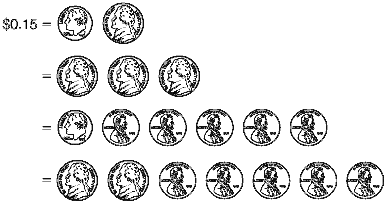
\includegraphics[scale=0.6]{img/change.png}
\caption{The four ways of getting 15 cents.  The dime and nickel combination is optimal.  \label{change}}
\end{figure}

It turns out for this problem, we can just pick the largest coin value possible, and repeat until done.  Because this algorithm takes the largest possible step to its goal every time (e.g. from 0 to 15), it is called \textit{greedy}. This produces the optimal solution for this particular set of coins, but does not work all the time.

\begin{problem}
You have $1\cent, 7\cent,$ and $9\cent$ coins.  Given some amount, $n$, provide the least number of coins which sum up to $n$.
\end{problem}

If we let $n=15$ again, then the first greedy choice takes the $9\cent$ coin.  There are $6\cent$ remaining, which must be made up for with $1 \cent$ coins.  This yields a 7 coin solution.  The optimal configuration is $7\cent,7\cent,1\cent$.

\subsection{Greedy methods}
Greedy methods apply to combinatorial optimization problems.  In these problems, we try to find some optimal set or combination of elements to minimize or maximize something given constraints.  In the previous case, the elements are coins, the constraints are that the coins sum to $n$, and we want to minimize the number of coins.

These problems pop up all over computer science, so we will spend some time studying them.

\subsubsection{Problems solved by greedy algorithms}

To determine if a greedy algorithm works for a problem, we need to show that the problem has the following properties:

\begin{itemize}
\item \textit{Greedy choice property}: an optimal solution contains the greedy choice.
\item \textit{Optimal substructure}: optimal solutions consists of an optimal subsolution, plus an optimal choice.
\end{itemize}

Change making contains optimal substructure.  Consider an optimal solution for $n$.  Then the coins making up $n-c$, where $c$ is an optimal choice, must have been optimal.  If it wasn't, then you can find some set to get less coins to make up $n-c$, and the original optimal solution was not optimal.

Change making does not contain the greedy choice property in general - as we've seen, sometimes the optimal solution does not contain the greedy choice.  However, in the US currency, it does.  If $n\ge25$, the optimal solution contains a quarter; if $n\ge10$, it contains a dime, etc.

We will not emphasize mathematical proofs in this course, but know that there is a method for determining when greedy algorithms can be applied.

\subsubsection{Properties of greedy algorithms}
Despite their limitations, it's worth noting greedy algorithms because when they do solve a problem, they are extremely efficient.  There is no backtracking, and they are easy to program.  Consider the following programs for the change-making problem.

Greedy solution:
\begin{verbatim}
sum, numcoins = 0
coins = [25,10,5,1]
while (sum < n)
  numcoins++
  for c in coins:
    if (n-sum >= c)
      sum = sum+c
\end{verbatim}

There is no algorithm more efficient.  You would have to build a tree-like structure for exhaustively searching the problem space.

\subsubsection{Drawbacks}
Greedy methods always take the largest step towards its goals, but in doing so may miss some better combinations, as seen in the second problem.  They do not take into account the future (if I take $7\cent$ instead of $9\cent$ now, then I can take another big coin in my next step).

However, even when greedy algorithms don't give the best result, sometimes the greedy choice is a good \textit{heuristic} for getting reasonable solutions (it can also be a very bad heuristic).  Some problems are intractable, and greedy algorithms can give decent answers in a reasonable time.

\subsection{Activity selection}
\begin{problem}
There are $n$ activities, each with start times $s_i$ and finish times $f_i$.  How do you pick a set of non-overlapping activities so that you perform the most possible activities?
\end{problem}

The solution, surprisingly, consists of picking the earliest ending activities, removing the overlapping activities, and repeat (see Figure \ref{activities}).

\begin{figure}
\centering
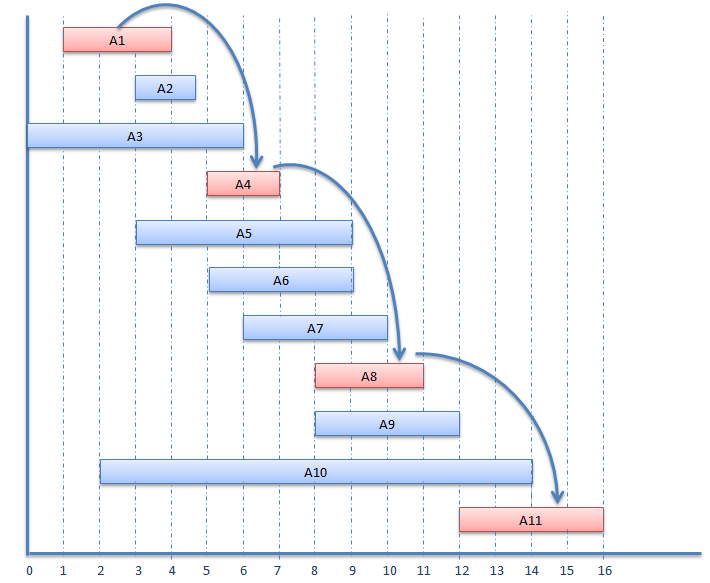
\includegraphics[scale=0.6]{img/activities.png}
\caption{A set of activities with finish and end times.  If we want to perform the most activities, A1, A4, A8, and A11 is optimal.  \label{activities}}
\end{figure}

We can prove that this greedy solution works.  Order the talks $a_i$ by finish time, so that $a_1$ is the first activity to finish.  

$a_1$ must be in \textit{some optimal solution}, because if a solution is optimal, then it must contain an event overlapping with $a_1$.  Since $a_1$ is the first activity, the overlapping event must start after $a_1$.  So we can replace the activity with $a_1$ and still have an optimal solution.  This proves the greedy choice property.

After removing the optimal choice, we are left with a set of maximal events.  We have to select the optimal set of events among this now reduced set.  Thus, the problem contains the optimal substructure property.

\section{Huffman Coding}
\subsection{Idea}
In ASCII encoding, each character is represented by 8 bits.  However, some letters are extremely rare, and some very common.  We can define an alternative mapping, where less common characters like 'z' require more than 8 bits, and more common characters like 's' take up less than 7 bits.  Using this encoding, we can save space.

However, with \textit{variable-length encoding}, we have to make sure no codes are prefices of one another.  For example, we cannot have "0" code to 'a', and "01" code to 'b', because we won't know whether to decode the "0" right away, or wait for more input.  There must be no ambiguity in parsing.  

These types of variable-length codes are called \textit{prefix codes}.  Because these codes consist of bits, we can represent them using a binary tree, as in Figure \ref{prefix}.  Each path in the tree represents a bit string.  Note that characters are leaves; if there was a character which descended from another character, then one code was a prefix of the other.

\begin{figure}
\centering
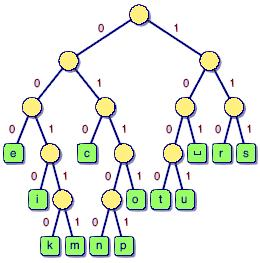
\includegraphics[scale=0.8]{img/prefix-code.jpg}
\caption{A tree representing prefix codes.  \label{prefix}}
\end{figure}

\subsection{Huffman codes}
Huffman codes solve the problem of finding the optimal encoding.  Note that the code depends on the text being compressed.

We want to have shorter codes / shorter paths / less parents for characters with very high counts, but we are alright with having many parents for characters with less counts.

\begin{enumerate}
\item Create a leaf node for each character, put them in priority queue in order of counts.
\item While the queue has more than one character:
\begin{itemize}
\item Remove two nodes with lowest counts.
\item Merge them to have one parent, with a cumulative sum.
\item Add this node to the queue.
\end{itemize}
\item Last node will be the root node.
\end{enumerate}

See Figure \ref{huffman} for a visual.

\begin{figure}
\centering
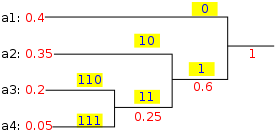
\includegraphics[scale=0.7]{img/huffman.png}
\caption{Huffman algorithm for combining characters a1, a2, a3, and a4.  Red numbers represent frequency, and yellow numbers represent code. \label{huffman}}
\end{figure}
Since efficient priority queue data structures require $O(\log n)$ time per insertion, and a tree with n leaves has $2n-1$ nodes, this algorithm operates in $O(n \log n)$ time, where n is the number of characters.

\subsection{Greediness of Huffman codes}
Huffman codes are greedy in the sense that the least frequent codes are given the longest paths in the tree.

Greedy choice property: if $x$ and $y$ have the two lowest counts, then the optimal algorithm will have them at the same path length, i.e. their codes are two of the longest.

Optimal substructure: every subtree of a Huffman code defines an optimal code for its leaf characters.

\end{document}